% Topic from _Linear Algebra_ Jim Hefferon
%  http://joshua.smcvt.edu/linalg.html
%  2012-Feb-12
\topic{Magic Squares}
\index{magic squares|(}
According to legend, 
in ancient China there was a flood in the Lo river.
The people offered sacrifices to the river, 
to appease him.
Each time from the river emerged a turtle, one of the celestial animals, 
and walked around the sacrifice.
Fuh-Hi (2858-2738~BC), the founder of Chinese civilization,  
interpreted this to say that
the river had not accepted the sacrifice.  
Then a child noticed that the turtle had on its shell what is today
known as the Lo Shu pattern.
\begin{center}
  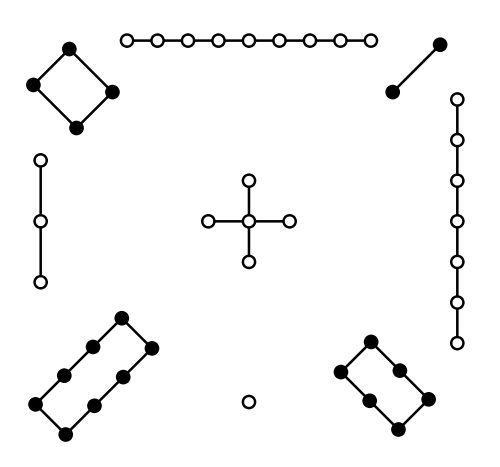
\includegraphics{LoShu.png}
\end{center}
Counting the dots gives a matrix.
\begin{center}
  \begin{tabular}{|c|c|c|}
    \hline
      $4$  &$9$  &$2$  \\ \hline
      $3$  &$5$  &$7$  \\ \hline
      $8$  &$1$  &$6$  \\ \hline    
  \end{tabular}
\end{center}
Each row, column, 
and diagonal adds to $15$
(the number of days in each of the twenty four cycles of the Chinese solar year).
Now that the people knew how much to sacrifice, they at last appeased the river.
(http://en.wikipedia.org/wiki/Lo_Shu_Square)

\textit{Melencolia I} is an engraving by Albrecht D\"urer.
(http://en.wikipedia.org/wiki/Melencolia_I)
\begin{center}
  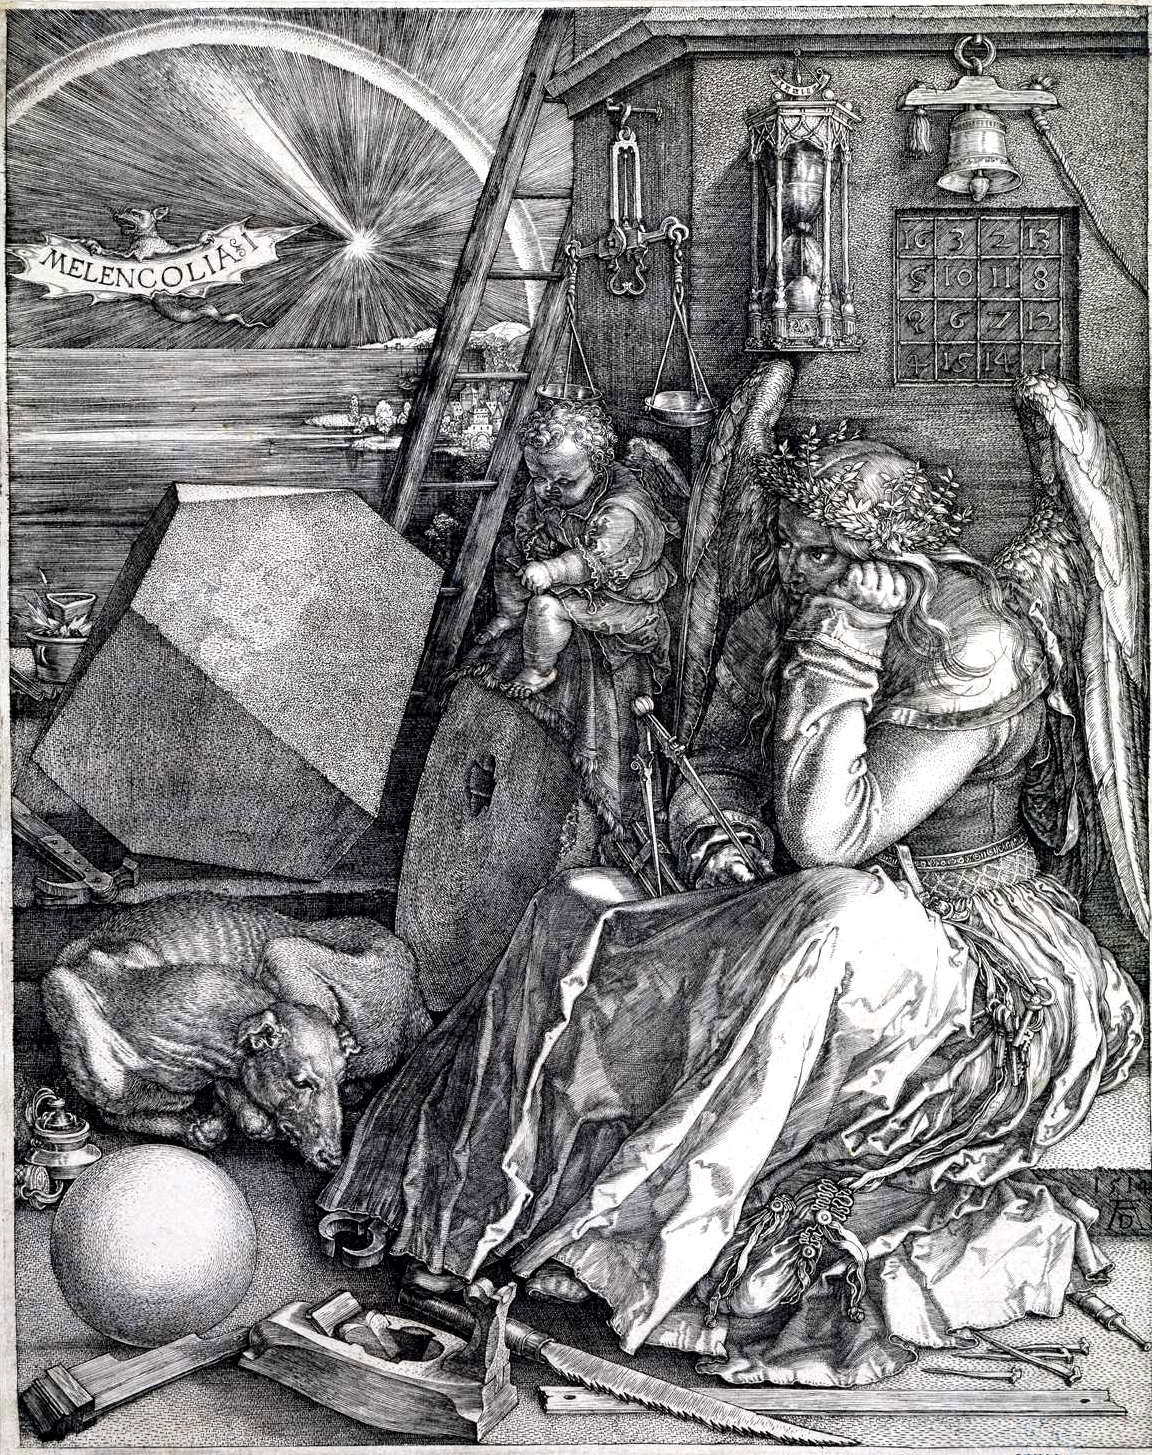
\includegraphics{Melencolia.jpg} % wikipedia http://upload.wikimedia.org/wikipedia/commons/1/14/Melencolia_I_%28Durero%29.jpg
\end{center}
One interpretation is that it depicts the melancholy or depressive state.
The figure, representing genius,
is surrounded by a wealth of fascinating things to be discovered an explored, 
including
the compass, the geometrical solid, the scale, and the hourglass.
But the figure seems unmoved; all the things are unused.
One of the potential delights is the $\nbyn{4}$ matrix in the upper right.
The rows, columns, and diagonals add to $34$.
\begin{center}
  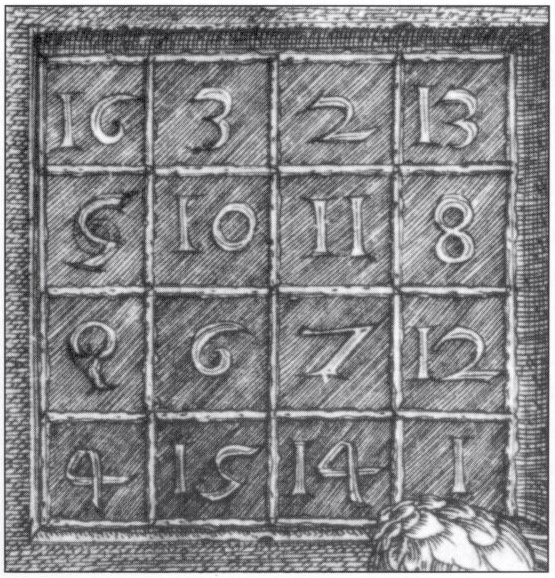
\includegraphics{Melencoliadetail.jpg} % wikipedia http://upload.wikimedia.org/wikipedia/commons/7/7e/Albrecht_D%C3%BCrer_-_Melencolia_I_%28detail%29.jpg
\end{center}
The middle entries on the bottom row give $1514$, the 
date of the engraving.

A \definend{magic square}\index{magic square}\index{matrix!magic square}
is a square matrix such that each row, column, and diagonal add to the same
value.

Every $\nbyn{1}$ square is magic.
For the $\nbyn{2}$ case, if the rows, columns, and diagonals add to $k$
\begin{equation*}
  \begin{mat}
    a  &b  \\
    c  &d
  \end{mat}
\end{equation*}
then $a+b=k$, $c+d=k$, $a+c=k$, $b+d=k$, $a+d=k$, and $b+c=k$.
That system has the unique solution $a=b=c=d=k/2$.




It is an unsolved problem to determine the number of magic squares of an arbitrary order, but the number of distinct magic squares (excluding those obtained by rotation and reflection) of order n=1, 2, ... are 1, 0, 1, 880, 275305224, ... (Sloane's A006052; Madachy 1979, p. 87). The 880 squares of order four were enumerated by Frénicle de Bessy in 1693, and are illustrated in Berlekamp et al. (1982, pp. 778-783). The number of 5×5 magic squares was computed by R. Schroeppel in 1973. The number of 6×6 squares is not known, but Pinn and Wieczerkowski (1998) estimated it to be (1.7745+/-0.0016)×10^(19) using Monte Carlo simulation and methods from statistical mechanics. 
(http://mathworld.wolfram.com/MagicSquare.html)


\begin{exercises}
  \item 
    Solve the system $a+b=k$, $c+d=k$, $a+c=k$, $b+d=k$, $a+d=k$, and $b+c=k$.
    \begin{answer}
      For any $k$ we have this.
      \begin{equation*}
        \begin{amat}{4}
          1  &1  &0  &0  &k  \\
          0  &0  &1  &1  &k  \\
          1  &0  &1  &0  &k  \\
          0  &1  &0  &1  &k  \\
          1  &0  &0  &1  &k  \\
          0  &1  &1  &0  &k            
        \end{amat}\;\grstep[-\rho_1+\rho_5]{-\rho_1+\rho_3}\;
        \begin{amat}{4}
          1  &1  &0  &0  &k  \\
          0  &0  &1  &1  &k  \\
          0  &-1 &1  &0  &0  \\
          0  &1  &0  &1  &k  \\
          0  &-1 &0  &1  &0  \\
          0  &1  &1  &0  &k            
        \end{amat}\;\grstep{-\rho_2\leftrightarrow\rho_6}\;
        \begin{amat}{4}
          1  &1  &0  &0  &k  \\
          0  &1  &1  &0  &k  \\          
          0  &-1 &1  &0  &0  \\
          0  &1  &0  &1  &k  \\
          0  &-1 &0  &1  &0  \\
          0  &0  &1  &1  &k  
        \end{amat}\;\grstep[-\rho_2+\rho_4 \\ \rho_2+\rho_5]{-\rho_2+\rho_3}\;
        \begin{amat}{4}
          1  &1  &0  &0  &k  \\
          0  &1  &1  &0  &k  \\          
          0  &0  &2  &0  &k  \\
          0  &1  &-1 &1  &0  \\
          0  &0  &1  &1  &k  \\
          0  &0  &1  &1  &k  
        \end{amat}
      \end{equation*}
      The unique solution is $a=b=c=d=k/2$.
    \end{answer}
\end{exercises}
\index{magic squares|)}
\endinput


